\documentclass[a4paper,11pt,openany]{book}
\usepackage{knowledge}

\title{Математические основы криптологии}
\author{Автор курса: Применко Эдуард Андреевич \\ 
		Составитель: Смирнов Дмитрий Константинович}
\date{Версия от \currenttime, \today}

\begin{document}

\maketitle
\tableofcontents

\mainmatter
\chapter{Домашние задания}

\include{mok/1-el-group}
\section{Квадратичные вычеты, сравнения, символ Лежандра.}

Докажем вспомогательные леммы.

\lemmata{Если $p = 2^m + 1$ -- простое и $\lege{a}{p} = -1$, то $\gen{a} = \mathbb{Z}^*_p$.}
\prove{
По определению первообразного корня достаточно доказать два утверждения: $\ a^{\phi(p)} = a^{2^m} \equiv 1 \pmod p$ и $\ a^{\frac{\phi(p)}{2}} = a^{2^{m-1}} \not \equiv 1 \pmod p.$

$$ a ^ {2 ^ {m - 1}} = a ^ {\frac{p - 1}{2}} = \lege{a}{p} = -1 \not \equiv 1 \pmod p, $$
$$a ^ {2^m} = (a ^ {2 ^ {m - 1}} )^2 = (-1)^2 = 1 \equiv 1 \pmod p. $$
}

\lemmata{Если число $p = 2^m + 1$ -- простое, $m > 1$, то $p \equiv 2 \pmod 3.$}
\prove{
По теореме о делении с остатком, число $p$ представимо в виде:
$$p = 3k + t, 0 \le t < 3.$$

\noindent Рассмотрим данное равенство при различных $t$.

а) $t = 0 \Rightarrow p = 3k$, то есть, $p$ не является простым числом при $k > 1$ (а значит, при $m > 1$). Противоречие $\Rightarrow t \ne 0$.

б) $t = 1 \Rightarrow 2^m = 3k$ -- этого не может быть ни при каком целом $k$ по лемме Евклида (по крайней мере один из сомножителей числа $2^m$ должен делиться на $3$). Следовательно, $t \ne 1$.

Тогда $t = 2$ -- единственный вариант, $p = 3k + 2$.
}

\lemmata{Если $p = 2^{2^n} + 1$, $n > 1$, то $p \equiv 2 \pmod 5.$}
\prove{
Докажем по индукции.

1) При $n = 2$ утверждение верно: $2^{2^2}+1 = 17 \equiv 2 \pmod 5$.

2) Пусть для $n = m$ верно, докажем для $n = m + 1$:
$$2^{2^{m+1}} + 1 = (2^{2^{m}} + 1 - 1)^2 + 1 = (2 - 1)^2 + 1 = 2 \equiv 2 \pmod 5.$$
}

\lemmata{Если $p = 2^{2^n} + 1$, $n = 2k$, то $p \equiv 3 \pmod 7.$}
\prove{
Докажем по индукции.

1) При $k = 0$ утверждение верно: $2^{2^0}+1 = 3 \equiv 3 \pmod 7$.

2) Пусть для $k = m$ верно, докажем для $k = m + 1$:
$$2^{2^{2(m+1)}} + 1 = (2^{2^{2m}} + 1 - 1)^4 + 1 = (3 - 1)^4 + 1 = 17 \equiv 3 \pmod 7$$
}

\lemmata{Если $p = 2^{2^n} + 1$, $n = 2k + 1$, то $p \equiv 5 \pmod 7.$}
\prove{
Докажем по индукции.

1) При $k = 0$ утверждение верно: $2^{2^1}+1 = 5 \equiv 5 \pmod 7$.

2) Пусть для $k = m$ верно, докажем для $k = m + 1$:
$$2^{2^{2(m+1)+1}} + 1 = (2^{2^{2m+1}} + 1 - 1)^4 + 1 = (5 - 1)^4 + 1 = 257 \equiv 5 \pmod 7$$
}

\task{Доказать, что сравнение $x^2 + 1 \equiv 0 \pmod p$ разрешимо тогда и только тогда, когда $p \equiv 1 \pmod 4$.}

$x^2 + 1 \equiv 0 \pmod p $ -- разрешимо $ \Leftrightarrow \lege{-1}{p} = 1 \Leftrightarrow (-1)^{\frac{p-1}{2}} = 1 \\ \Leftrightarrow \frac{p-1}{2} = 2k \Leftrightarrow p = 4k + 1 \Leftrightarrow p \equiv 1 \pmod 4$

\task{Доказать, что сравнение $x^2 + 2 \equiv 0 \pmod p$ разрешимо тогда и только тогда, когда $p = 1, 3 \pmod 8$.}

$x^2 + 2 \equiv 0 \pmod p $ -- разрешимо $ \Leftrightarrow \lege{-2}{p} = 1. \Leftrightarrow \big \{ \lege{-2}{p} = \lege{-1}{p} \cdot \\ \cdot \lege{2}{p} = (-1)^{\frac{p-1}{2}} \cdot (-1)^{\frac{p^2-1}{8}} \big \} \Leftrightarrow \frac{p-1}{2} + \frac{p^2-1}{8} = 2k \Leftrightarrow p^2 + 4p - 16k - 5 = 0.$

Представим $p$, используя теорему о делении с остатком, в следующем виде: $p = 8m + t,\ 0 \le t < 8$. Решим полученную систему относительно $t$.

$(8m + t)^2 + 4(8m + t) - 16k -5 = 0$

$ t^2 + (16k + 4)t + 64k^2 + 32k - 16m - 5 = 0$

$t_{1, 2} = -8k - 2 \pm \sqrt{16m + 9} \pmod 8 = -2 \pm 3 \pmod 8 \Rightarrow t = 1,3$ \\

\noindent Тогда $p^2 + 4p - 16k - 5 = 0 \Leftrightarrow p = 1, 3 \pmod 8$.

\task{Доказать, что сравнение $x^2 + 3 \equiv 0 \pmod p$ разрешимо тогда и только тогда, когда $p \equiv 1 \pmod 6$.}

Пусть $p = 3k + t, t < 3.$

$x^2 + 3 \equiv 0 \pmod p \Leftrightarrow \lege{-3}{p} = 1.$

$ \lege{-3}{p} = \lege{-1}{p} \lege{3}{p} = (-1)^{\frac{p-1}{2}}(-1)^{\frac{p-1}{2} \cdot \frac{3-1}{2}} \lege{p}{3} = (-1)^{3k + t -1} \lege{t}{3}$\\

а) $t = 0 \Rightarrow \lege{0}{3} = 0$, $(-1)^{3k + t -1} \lege{t}{3} = 0 \ne 1$

б) $t = 1 \Rightarrow \lege{1}{3} = 1$, $(-1)^{3k + t -1} \lege{t}{3} = (-1)^{3k} \cdot 1 = (-1)^{3k}$.

в) $t = 2 \Rightarrow \lege{2}{3} = -1$, $(-1)^{3k + t -1} \lege{t}{3} = (-1)^{3k + 1} \cdot (-1) = (-1)^{3k}$ \\

$(-1)^{3k} = 1 \Leftrightarrow k = 2m \Leftrightarrow p = 6m + 1 \Leftrightarrow p \equiv 1 \pmod 6$

\task{Доказать, что если $p = 2^n + 1$ -- простое, $n > 2$, то $\lege{3}{p} = -1$ и $\gen{3} = \mathbb{Z}^*_p$.}

$p = 3k + 2$ по лемме 2.2. 

$ \lege{3}{p} = (-1)^{\frac{3-1}{2} \cdot \frac{2^n + 1 -1}{2}} \lege{p}{3} = (-1)^{2^{n - 1}} \lege{2}{3} = -1$ \\

Выполнены все условия леммы 2.1 $\Rightarrow \gen{3} = \mathbb{Z}^*_p$.

\task{Доказать, что если $p = 2^n + 1$ -- простое и $\lege{a}{p} = -1$, то $\gen{a} = \mathbb{Z}^*_p$.}

Доказано в качестве леммы 2.1.

\task{Доказать, что если $p = 4q + 1$, $p$ и $q$ -- простые, то $\gen{2} = \mathbb{Z}^*_p$.}

По определению первообразного корня достаточно доказать три утверждения: \\ 1) $2^{\phi(p)} = 2^{4q} \equiv 1 \pmod p$,\\ 2)$\ 2^{\frac{\phi(p)}{2}} =  2^{2q} \not \equiv 1 \pmod p$, \\ 3) $2^{\frac{\phi(p)}{q}} =  2^{4} \not \equiv 1 \pmod p$.

Начнём с третьего. Представим $2^4$ в следующем виде: $2^4 = pk + t, \\ 0 \le t < p$. Значит, нам нужно доказать, что $t \ne 1$. Предположим, что это не так, тогда $pk = 2^4 - 1 = 15$. Обратим внимание на условие: если и $p$, и $q$ -- простые числа, то $p$ не может быть ни 3, ни 5. Значит, в левой части равенства содержится простой множитель, которого нет в правой части. Мы получили противоречие, а значит, $t \ne 1 \Rightarrow 2^{\frac{\phi(p)}{q}} =  2^{4} \not \equiv 1 \pmod p$.

Рассмотрим теперь второе утверждение. Заметим, что:

$$\lege{2}{4q + 1} = 2 ^ {\frac{4q + 1 - 1}{2}} = 2 ^ {2q} \pmod {4q + 1}.$$

Вычислим $\lege{2}{4q+1} = (-1) ^ {\frac{(4q+1)^2 - 1}{8}} = (-1)^{2q^2 + q} = \big\{q$ -- нечет$\big\} = -1$. Тем самым мы доказали второе утверждение.

Поскольку $2^{4q} = (2^{2q})^2 = (-1)^2 = 1 \pmod {4q+1}$, то первое утверждение становится следствием второго.

\task{Доказать, что если $p = 2^{2^n} + 1$ -- простое и $\lege{a}{p} = -1$, то $\gen{a} = \mathbb{Z}^*_p$.}

Приняв $m = 2^n$ в лемме 2.1, получим справедливость данного утверждения.


\task{Доказать, что если $p = 2^{2^n} + 1$ -- простое, $n>2$, то $\gen{3} = \gen{5} = \gen{7} = \mathbb{Z}^*_p$.}

Покажем $\lege{3}{p} = \lege{5}{p} = \lege{7}{p} = -1$.

$2^{2^n} + 1 = 3k + 2$ по лемме 2.2.
$$\lege{3}{p} = (-1) ^ {\frac{3 - 1}{2} \cdot \frac{2^{2^n} + 1 - 1}{2}} \lege{p}{3} = (-1) ^ {2^{2^n - 1}} \lege{3k+2}{3} = \lege{2}{3} = 2^{\frac{3-1}{2}} \pmod 3 = -1$$

$2^{2^n} + 1 = 5k + 2$ по лемме 2.3.
$$\lege{5}{p} = (-1) ^ {\frac{5 - 1}{2} \cdot \frac{2^{2^n} + 1 - 1}{2}} \lege{p}{5} = (-1) ^ {2^{2^n}} \lege{5k+2}{5} = \lege{2}{5} = 2^{\frac{5-1}{2}} \pmod 5= -1$$

$2^{2^n} + 1 = 7k + 3,\ n = 2t$ по лемме 2.4.

$$\lege{7}{p} = (-1) ^ {\frac{7 - 1}{2} \cdot \frac{2^{2^n} + 1 - 1}{2}} \lege{p}{7} = (-1) ^ {2^{2^n}} \lege{7k+3}{7} = \lege{3}{7} = 3^{\frac{7-1}{2}} \pmod 7 = -1$$

$2^{2^n} + 1 = 7k + 5,\ n = 2t + 1$ по лемме 2.5.

$$\lege{7}{p} = \lege{5}{7} = 5^{\frac{7-1}{2}} \pmod 7 = -1.$$

Осталось применить лемму 2.1, и исходное утверждение будет доказано. 

\section{Рекуррентные последовательности.}
\task{$F = GF(5)$. Построить граф отображения и найти период РП, заданной характеритической функцией:
$$x_i = x_{i-1} + 2 x_{i-2} x_{i-1} + 2.$$
Начальное заполнение: $12=\gamma_1 + 5 \gamma_2$ ($\gamma = (2, 2)$).
}

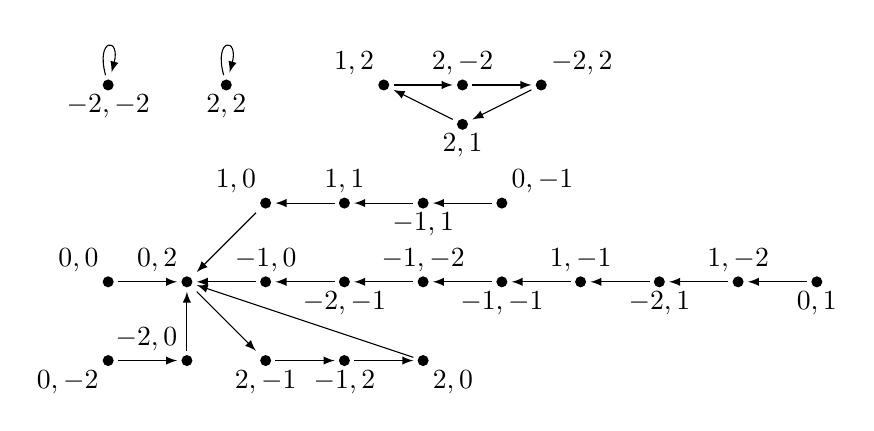
\begin{tikzpicture}[>=latex]
{\centering
\node (-2-2) at (-0.5, 2)    {};
\node (-2-1) at (2.5, -0.5)   {};
\node (-20) at (0.5, -1.5) {};
\node (-1-2) at (3.5, -0.5)   {};
\node (-1-1) at (4.5, -0.5) {};
\node (-10) at (1.5, -0.5)   {};
\node (0-2) at (-0.5, -1.5)   {};
\node (0-1) at (4.5, 0.5) {};
\node (00) at (-0.5, -0.5)    {};
\node (1-2) at (7.5, -0.5) {};
\node (1-1) at (5.5, -0.5)  {};
\node (10) at (1.5, 0.5) {};
\node (2-2) at (4, 2)   {};
\node (2-1) at (1.5, -1.5) {};
\node (20) at (3.5, -1.5) {};

\node (-22) at (5, 2)    {};
\node (-21) at (6.5, -0.5)  {};
\node (-12) at (2.5, -1.5)   {};
\node (-11) at (3.5, 0.5) {};
\node (02) at (0.5, -0.5)   {};
\node (01) at (8.5, -0.5) {};
\node (12) at (3, 2) {};
\node (11) at (2.5, 0.5)   {};
\node (22) at (1, 2)   {};
\node (21) at (4, 1.5) {};

\fill (-2-2)[right] circle (0.07) node[below]       {$-2,-2$};
\fill (-2-1)[right] circle (0.07) node[below]       {$-2,-1$};
\fill (-20)[left] circle (0.07) node[above left]       {$-2,0$};
\fill (-21)[left] circle (0.07) node[below]       {$-2,1$};
\fill (-22)[left] circle (0.07) node[above right]       {$-2,2$};
\fill (-1-2)[left] circle (0.07) node[above]       {$-1,-2$};
\fill (-1-1)[left] circle (0.07) node[below]  {$-1,-1$};
\fill (-10)[left] circle (0.07) node[above]       {$-1,0$};
\fill (-11)[left] circle (0.07) node[below]  {$-1,1$};
\fill (-12)[left] circle (0.07) node[below]  {$-1,2$};
\fill (0-2)[left] circle (0.07) node[below left]  {$0,-2$};
\fill (0-1)[left] circle (0.07) node[above right]       {$0,-1$};
\fill (00)[left] circle (0.07) node[above left]       {$0,0$};
\fill (01)[left] circle (0.07) node[below]  {$0,1$};
\fill (02)[left] circle (0.07) node[above left] {$0,2$};
\fill (2-2)[right] circle (0.07) node[above]       {$2,-2$};
\fill (2-1)[right] circle (0.07) node[below ]       {$2,-1$};
\fill (20)[left] circle (0.07) node[below right]       {$2,0$};
\fill (21)[left] circle (0.07) node[below]       {$2,1$};
\fill (22)[left] circle (0.07) node[below]       {$2,2$};
\fill (1-2)[left] circle (0.07) node[above]       {$1,-2$};
\fill (1-1)[left] circle (0.07) node[above]  {$1,-1$};
\fill (10)[left] circle (0.07) node[above left]       {$1,0$};
\fill (11)[left] circle (0.07) node[above]  {$1,1$};
\fill (12)[left] circle (0.07) node[above left]  {$1,2$};

%>>> def f(x1, x2):
%...     y = (x2 + 2 * x1 * x2 + 2) % 5
%...     return y if y < 3 else y - 5

%>>> d = {(x, y): (y, f(x, y)) for x in range(-2, 3) for y in range(-2, 3)}
%>>>for k in d:
%...     if k == d[k]:
%...             print('\path[->]', k, 'edge [loop above] node {} ();')
%...     else:
%...             print('\path[->]', k, 'edge node {}', d[k], ';')

\path[->] (-2-2) edge [loop above] node {} ();
\path[->] (-2-1) edge node {} (-10) ;
\path[->] (-20) edge node {} (02) ;
\path[->] (-21) edge node {} (1-1) ;
\path[->] (-22) edge node {} (21) ;
\path[->] (-1-2) edge node {} (-2-1) ;
\path[->] (-1-1) edge node {} (-1-2) ;
\path[->] (-10) edge node {} (02) ;
\path[->] (-11) edge node {} (11) ;
\path[->] (-12) edge node {} (20) ;
\path[->] (0-2) edge node {} (-20) ;
\path[->] (0-1) edge node {} (-11) ;
\path[->] (00) edge node {} (02) ;
\path[->] (01) edge node {} (1-2) ;
\path[->] (02) edge node {} (2-1) ;
\path[->] (1-2) edge node {} (-21) ;
\path[->] (1-1) edge node {} (-1-1) ;
\path[->] (10) edge node {} (02) ;
\path[->] (11) edge node {} (10) ;
\path[->] (12) edge node {} (2-2) ;
\path[->] (2-2) edge node {} (-22) ;
\path[->] (2-1) edge node {} (-12) ;
\path[->] (20) edge node {} (02) ;
\path[->] (21) edge node {} (12) ;
\path[->] (22) edge [loop above] node {} ();

}
\end{tikzpicture}

В случае $\gamma = (2, 2)$ последовательность оказывается полностью состоящей из двоек, поэтому период такой последовательности будет равен единице.

\task{Над полем $GF(2)$ построить ЛРП периода $T$ и ранга $n$ и указать начальное заполнение.

$T = 84, n = 8.$
}

Разложим $T$ на множители: $T = 84 = 4 \cdot 3 \cdot 7$. 

ЛРП$_1$ c периодом 4 соответствует минимальный многочлен
$$f_1 (x) = x^3 + x^2 + x + 1,\ x_i = x_{i-1} + x_{i-2} + x_{i-3}.$$

ЛРП$_2$ с периодом 3 соответствует минимальный многочлен
$$f_2 (x) = x^2 + x + 1,\ x_i = x_{i-1} + x_{i-2}.$$

ЛРП$_3$ с периодом 7 соответствует минимальный многочлен
$$f_3 (x) = x^3 + x + 1,\ x_i = x_{i-2} + x_{i-3}$$

Искомый характеристический многочлен
$$f(x) = (x^3 + x^2 + x + 1)(x^2 + x + 1)(x^3 + x + 1) = x^8 + x^4 + x^3 + x^2 + x + 1.$$

Характеристическое уравнение будет иметь вид:
$$x_i = x_{i-4} + x_{i-5} + x_{i-6} + x_{i-7} + x_{i-8}.$$

Выберем начальные заполнения для ЛРП$_{1-3}$, отличные от нуля, и получим первые начальные отрезки ЛРП длины $n=8$:
$$\widetilde \alpha _1 = 001 \Rightarrow \widetilde \beta _1 = 00110011$$
$$\widetilde \alpha _2 = 01 \Rightarrow \widetilde \beta _2  = 01101101$$
$$\widetilde \alpha _3 = 001 \Rightarrow \widetilde \beta _3 = 00101110$$

Искомое начальное заполнение:
$$\widetilde \beta = \widetilde \beta _1 \oplus \widetilde \beta _2 \oplus \widetilde \beta _3 = 01110000.$$

Ответ: $f(x) = x^8 + x^4 + x^3 + x^2 + x + 1$, $\widetilde \beta = 01110000$. 

\section{Шифр гаммирования}
\task{Зашифровать свою фамилию, используя шифр гаммирования с ЛРП из задачи 3.2.}

Кодирование алфавита приведено в следующей таблице:
\medskip

{\centering
\begin{tabular}{||c|c||c|c||c|c||c|c||}
\hline
А & 00000 & И & 01000 & Р & 10000 & Ш & 11000 \\
\hline
Б & 00001 & Й & 01001 & С & 10001 & Щ & 11001 \\
\hline
В & 00010 & К & 01010 & Т & 10010 & Ъ & 11010 \\
\hline
Г & 00011 & Л & 01011 & У & 10011 & Ы & 11011 \\
\hline
Д & 00100 & М & 01100 & Ф & 10100 & Ь & 11100 \\
\hline
Е & 00101 & Н & 01101 & Х & 10101 & Э & 11101 \\
\hline
Ж & 00110 & О & 01110 & Ц & 10110 & Ю & 11110 \\
\hline
З & 00111 & П & 01111 & Ч & 10111 & Я & 11111 \\
\hline
\end{tabular}

}

\medskip

ЛРП задана многочленом $f(x) = x^8 + x^4 + x^3 + x^2 + x + 1$, $\widetilde k = 01110000$, $M = СМИРНОВ$. Согласно кодовой таблице получим:

$$\widetilde M = 10001\ 01100\ 01000\ 10000\ 01101\ 01110\ 00010$$

Получаем гамму:

$$\widetilde \Gamma = 01110\ 00011\ 01100\ 10101\ 00010\ 01011\ 00011$$

Получим шифротекст:

$$\widetilde T = 11111\ 01111\ 00100\ 00101\ 01111\ 00101\ 00001$$

Представим его в буквенном виде.

Ответ: $T = ЯПДЕПЕБ$.
\section{Теория групп}

\task{Определить структуру группы $\mathbb{Z}^*_n$ , разложить её в прямое произведение циклических подгрупп и подсчитать число элементов различного порядка, $n = 84$.}

$|G| = \phi (84) = \phi (2^2) \cdot \phi (3) \cdot \phi (7) = (4 - 2)(3 - 1)(7 - 1) = 24 = 2^3 \cdot 3$.

\noindent Следовательно, $G \cong S_1(8) \times S_2 (3)$.

1.  Определим структуру примарной группы $S_1(8)$. Для этого нужно решить сравнение:

$$x^2 \equiv 1 \pmod{84}.$$

По КТО это равносильно следующей системе:

\begin{equation*}
	\begin{cases}
	x^2 \equiv 1 \pmod 3 \\
	x^2 \equiv 1 \pmod 4 \\
	x^2 \equiv 1 \pmod 7
	\end{cases}
\end{equation*}

$p = 3 = 4 \cdot 0 + 3 \Rightarrow \lege{1}{3} = 1$ -- два решения: $x_1 \equiv \pm 1^{0+1} \pmod 3$.

$p = 4 = 2^2,\ a = 1 \Rightarrow $ два решения: $x_2 = \pm 1 \pmod 4$.

$p = 7 = 4 \cdot 1 + 3 \Rightarrow \lege{1}{7} = 1$ -- два решения: $x_3 \equiv \pm 1^{1+1} \pmod 7$.

Общее решение системы по КТО будет равно:

\begin{multline*}
X = x_1 (4 \cdot 7)[(4 \cdot 7)^{-1} \pmod 3] + x_2 (3 \cdot 7)[(3 \cdot 7)^{-1} \pmod 4] + \\
+ x_3 (3 \cdot 4)[(3 \cdot 4)^{-1} \pmod 7] \pmod {84} =
28 x_1 + 21 x_2 + 36 x_3 \pmod {84}
\end{multline*}

Таким образом, множество элементов второго порядка группы $G$ это:

$$M_2 = \{13, 43, 55, 29, 41, 71, 83\}.$$

Обозначим за $A_i = \left\langle M_{2, i} \right\rangle $, где $M_{2, i}$ -- $i$-тый элемент множества $M_2$. Тогда $S_1(8) \cong A_i \times A_j \times A_k$, $i, j, k = \overline{1, 7} $.

2. Определим структуру примарной группы $S_2(3)$. Для этого нужно решить сравнение:

$$x^3 \equiv 1 \pmod{84}.$$

По КТО это равносильно следующей системе:

\begin{equation*}
	\begin{cases}
	x^3 \equiv 1 \pmod 3 \\
	x^3 \equiv 1 \pmod 4 \\
	x^3 \equiv 1 \pmod 7
	\end{cases}
\end{equation*}

Первые два сравнения, очевидно, имеют единственные решения $x_1 =~1$, $x_2 = 1$. Последнее сравнение имеет 3 решения: $x_3 = \{1, 2, 4\}$. Общее решение исходного сравнения будет равно:

$$X = 28 x_1 + 21 x_2 + 36 x_3 \pmod {84} = 49 + 36 x_3 \pmod {84}$$

Множество элементов третьего порядка группы $G$ это:

$$M_3 = \{25, 37\}$$

Таким образом, $S_2(3) = \left\langle 25 \right\rangle = \left\langle 37 \right\rangle$. \\

\noindent Ответ: $G \cong A_i \times A_j \times A_k \times \left\langle 25 \right\rangle = A_i \times A_j \times A_k \times \left\langle 37 \right\rangle$, $i, j, k = \overline{1, 7}$. 

%\chapter{Экзамен}
\noindent \textit{1. Определение шифра. Шифр простой замены, перестановки, гаммирования. Основные условия криптоанализа.} \\

Отображение $T: X \times K \rightarrow Y$ называется \textbf{шифром}, если $\forall k \in K \\ \exists T^{-1} (y, k) = x$.

Пусть $A = \{ a_1, \ldots , a_m \}$ -- конечный алфавит, $S_m$ -- множество всех подстановок на $A$. Для некоторого натурального $n$ положим $X = A^n$. Если $x = (a_{i_1}, \ldots, a_{i_n})$, $k \in S_m$, то определим \textbf{шифр простой замены} следующим образом:
$$T(x, k) = (k(a_{i_1}), k(a_{i_2}), \ldots, k(a_{i_n})) = y = (b_{i_1}, \ldots, b_{i_n}).$$

Пусть $A = \{ a_1, \ldots , a_m \}$ -- конечный алфавит, $n$ -- натуральное число, $S_n$ -- симметрическая группа подстановок на множестве $\{1, \ldots, n\}$, $X =~A^n$. Если $x = (a_{i_1}, \ldots, a_{i_n})$, $k = \bigl(\begin{smallmatrix}
    1 & \cdots & n \\
    j_1 & \cdots & j_n
  \end{smallmatrix}\bigr) \in S_n$, то \textbf{шифр перестановки} на $X$ определяется следующим образом:
$$T(x, k) = (a_{i_{j_1}}, a_{i_{j_2}}, \ldots, a_{i_n}) = y.$$

Пусть $A = \{ 0, \ldots , m - 1 \}$ -- алфавит, $X =A^n$ -- множество открытых текстов. Рассмотрим кольцо вычетов $\mathbb{Z}_m$. Положим $K = A^n$ и $\forall x \in X, k \in K$, определим \textbf{шифр гаммирования}:
$$y = T(x, k) = (x + k) \pmod m,$$

\noindent где сложение происходит в кольце $\mathbb{Z}_m$.

\newpage
\textbf{Основные условия криптоанализа}:

\noindent 1. Известен шифртекст $y$, один или несколько. Задачи:

а) Нахождение $T$ -- преобразования зашифрования;

б) Нахождение $T, T^{-1}, x$ -- дешифрование по шифртексту.

\noindent 2. Известны одна или несколько пар $(x, y)$. Определить $T(T^{-1})$ и найти $k$ -- ключ шифрования.

\noindent 3. Известны $T(T^{-1})$, один или несколько шифртекстов y. Найти:

а) x -- бесключевое чтение;

б) k, x -- дешифрование по шифртексту при известной шифрсистеме.

\noindent 4. Известны $T, T^{-1}, (x, y)$. Найти $k$.

а) Известны особые x -- атака выбранного открытого текста;

а) Известны особые y -- атака с использованием шифртекста.

\noindent 5. Известны $T, T^{-1}$, шифртекст $y$ или пары $(x, y)$, некоторая форма преобразования $T(.,k)$, но неизвестны $k$ и $T^{-1}(., k)$ -- системы с открытым ключом (Диффи и Хеллман, 1976 г.) \\

\noindent \textit{2. Теоретическая стойкость по Шеннону. Практическая стойкость. Пример совершенного шифра.} \\

\textbf{Теоретическая стойкость} (совершенная секретность) -- Система является безопасной против атак противника с неограниченным временем и ресурсами.

\textbf{Практическая стойкость} (вычислительная) -- Система является безопасной против атак противника в ограниченный период времени с ограниченными ресурсами.

Шеннон определил совершенную секретность условием:
$$P(x | y) = P(x)\ \ \forall x \in X, y \in Y,$$
\noindent где $X, Y$ -- множества открытых сообщений и возможных шифртекстов.

\textbf{Пример совершенного шифра} -- шифр гаммирования, в котором равновероятный ключ имеет ту же длину, что и открытый текст. Пусть $X = \{0, 1\},\ Y = \{0, 1\}, K = \{0, 1\}$, $T(x, k) = (x \oplus k) \pmod 2$, \\ $T^{-1}(y, k) = (y \oplus k) \pmod 2$, $X \sim \begin{pmatrix}
    0 & 1 \\
    p & q
  \end{pmatrix}$, $q = 1 - p$, $Y \sim \begin{pmatrix}
    0 & 1 \\
    0.5 & 0.5
  \end{pmatrix}$, $K \sim \begin{pmatrix}
    0 & 1 \\
    0.5 & 0.5
  \end{pmatrix}$, $P(Y|X) = \frac{P(X, Y)}{P_X (X)} = \begin{pmatrix}
    y/x & 0 & 1 \\
    0 & 0.5 & 0.5 \\
    1 & 0.5 & 0.5 
  \end{pmatrix}$.

По формуле Байеса:
$$P(X = x | Y = y) = \frac{P_X(x) P(y | x)}{P(y)} = \frac{P_X(x)}{\frac{1}{2} 2} = P_X(x).$$

\noindent \textit{3. Метод полного перебора, его средняя трудоемкость. Параллельное опробование с помощью случайно выбираемого на каждом шагу ключа.} \\

Пусть известны $T, T^{-1}, (x, y)$, а ключ неизвестен. \textbf{Методом полного перебора} называется поиск решения уравнения $T(x, k) = y$ перебором по всем $k \in K,\ \ |K| < \infty$.

Определим случайные величины: $\tau$ -- количество опробований ключа включительно до момента обнаружения, $\xi_i = [$ключ на $i$-м месте$]$. Ключ равновероятен, тогда $P(\xi_i = 1) = \frac{1}{|K|}$ для всех $i = \overline{1, |K|}$. \textbf{Средняя трудоёмкость МПП}:
$$\mathbb{E} \tau = \sum_{i = 1}^{|K|} i P (\xi_i = 1)= \frac{1}{|K|} \sum_{i = 1}^{|K|} i = \frac{|K|(|K| + 1)}{|K| \cdot 2} = \frac{|K| + 1}{2}.$$

Пусть параллельно работают $N$ машин. Если $t$ -- число шагов работы машин, то $Nt$ -- число опробований. Число тактов опробования -- случайная величина $\eta$. Аналогом является задача о размещениях: в каждую из $|K|$ ячеек может попасть от $0$ до $N$ частиц. Вероятность того, что из комплекта $i$ ни одна частица не попадёт в данную ячейку, равна $q = (1 - \frac{1}{|K|})^N$. Первое попадание в данную ячейку на комплекте с номером $t$, означающее, что ключ получен, имеет вероятность $P(\eta = t) = q^{t-1}(1-q)$ -- с.в. $\eta$ имеет геометрическое распределение. Тогда \textbf{средняя трудоёмкость МПП при параллельном опробовании} равна: 
$$\mathbb{E}\eta = \frac{1}{1 - q} = \frac{1}{1 - (1 - \frac{1}{|K|})^N} \approx \big \{ N << |K| \big \} \approx \frac{1}{1 - 1 + \frac{N}{|K|}} = \frac{|K|}{N}.$$

\noindent \textit{4. Аналитический метод криптоанализа. Треугольные системы и их решение. Линейные системы. Сложность решения методом Гаусса.} \\

Пусть $K = K_1 \times K_2 \times \ldots \times K_r$, $x = (x_1 x_2 \ldots x_s)$, $y = (y_1 y_2 \ldots y_s)$, $x_i, y_i \in A$. \textbf{Идея аналитического метода} заключается в том, чтобы записать систему уравнений и решить её относительно ключа:

\begin{equation*}
    \begin{cases}
    y_1 = f_1 (x_1, \ldots, x_s, k_1, \ldots, k_r) \\
    \cdots \\
    y_s = f_s (x_1, \ldots, x_s, k_1, \ldots, k_r) 
    \end{cases}
\end{equation*}

\noindent Известны $f_i$ и $(x, y)$.

Пусть эту систему можно преобразовать к \textbf{треугольной системе}:

\begin{equation*}
    \begin{cases}
    g_1 (x, y) = h_1 (x, y, k_1) \\
    g_2 (x, y) = h_2 (x, y, k_1, k_2) \\
    \cdots \\
    g_r (x, y) = h_r (x, y, k_1, \ldots, k_r) 
    \end{cases}
\end{equation*}

\noindent 1. Опробуем $k_1 \in K_1$, число опробований $\le |K_1| \Rightarrow$ восстанавливаем $k_1$.

\noindent 2. Опробуем $k_2 \in K_2$, число опробований $\le |K_2| \Rightarrow$ восстанавливаем $k_2$.

\noindent \ldots

\noindent r. Опробуем $k_r \in K_r$, число опробований $\le |K_r| \Rightarrow$ восстанавливаем $k_r$. \\

\noindent Таким образом, сложность $\le |K_1| + |K_2| + \ldots + |K_r|$. \\

Пусть имеется \textbf{линейная система}:

\begin{equation*}
    \begin{cases}
    b_{11} k_1 + b_{12} k_2 + \ldots + b_{1r} k_r = g_1 (x, y)  \\
    b_{21} k_1 + b_{22} k_2 + \ldots + b_{2r} k_r = g_2 (x, y)  \\
    \cdots \\
    b_{r1} k_1 + b_{r2} k_2 + \ldots + b_{rr} k_r = g_r (x, y)  \\
    \end{cases}
\end{equation*}

\noindent Методом Гаусса решается за $\sum_{k=1}^r k^2 = \frac{r(r + 1)(2 r + 1)}{6} \approx \frac{r^3}{3}$ операций. \\

\noindent \textit{5. Регистр сдвига с нелинейной обратной связью. Линейная сложность. Условия регулярности (теорема с доказательством).} \\

Последовательность $\gamma$ называется \textbf{линейной рекуррентной последовательностью} (ЛРП) порядка $r > 0$ над $GF(2)$, если она описывается \textbf{законом рекурсии}:
$$\gamma_{n+r} = \sum_{i=0}^{r-1} \alpha_i \gamma_{r+n-i},\ \ n = 0,1,\ldots$$
\noindent $\alpha_i \in GF(2),\ i=1,\ldots,r-1,\ \alpha_0 = 1$ и все операции выполняются в поле $GF(2)$.

\textbf{Нелинейная рекуррентная последовательность} (НЛРП) определяется выражением:
$$\gamma_{n+r} = f (\gamma_n, \gamma_{n+1}, \ldots, \gamma_{n+r-1}),\ \ n = 0,1,\ldots$$

\textbf{Регистр сдвига с нелинейной обратной связью} (НЛРС) выглядит следующим образом:

\medskip

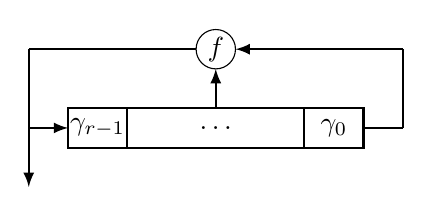
\begin{tikzpicture}[>=latex]
    {\centering
    
    \draw[thick] (0, 0) rectangle node[midway] {$\gamma_{r-1}$} (0.75, 0.5);

    \draw[thick] ( 0.75, 0) rectangle node[midway] {$\ldots$} (3 * 0.75 + 0.75, 0.5);
    \draw[thick, ->] (0.375 + 2 * 0.75, 0.5) -- (0.375 + 2 * 0.75, 1);

    \draw[thick] (4 * 0.75, 0) rectangle node[midway] {$\gamma_0$} (4 * 0.75 + 0.75, 0.5);

    \draw[thick, <-] (0,0.25) -- (-0.5,0.25);
    \draw[thick, <-] (-0.5, -0.5) -- (-0.5,1.25);
    \draw[thick, -] (-0.5,1.25) -- (1.875 - 0.25,1.25);
    
    \draw (1.875, 1.25) circle (0.25) node {$f$};
    
    \draw[thick, -] (3.75, 0.25) -- (4.25,0.25);
    \draw[thick, -] (4.25, 0.25) -- (4.25,1.25);
    \draw[thick, <-] (1.875 + 0.25,1.25) -- (4.25,1.25);

    }
\end{tikzpicture}

\medskip

Нелинейный регистр сдвига называется \textbf{регулярным}, если порождаемая им выходная последовательность $\gamma$ периодична при любом начальном заполнении регистра.

\textbf{Условие регулярности}: если НЛРС регулярен, то для любого начального заполнения существует ЛРС (вида) размера $v$ ($v \ge r$) такой, что порождаемая им последовательность совпадает с последовательностью, порождаемой при этом начальном заполнении НЛРС.

\textbf{Доказательство}: НЛРС регулярен $\Rightarrow$ при любом начальном заполнении последовательность $\gamma$ периодична $\Rightarrow$ ЛРС вида $\gamma_{n+T} = \gamma_n,\\ n = 0, 1, \ldots$ порождает ту же последовательность. \\

\noindent \textit{6. Метод “встреча посередине”. Трудоемкость метода. Пример реализации метода “встреча посередине”.} \\

Пусть даны два шифра: $T_1 (x, k_1)$ и $T_2 (z, k_2)$. Положим
$$y = T_2 (T_1 (x, k_1), k_2)$$

\noindent \textit{9. Первая теорема Шеннона (теорема с доказательством).} \\



\noindent \textit{10. Вторая теорема Шеннона (теорема с доказательством).} \\




\end{document}